\section{Appendix 1 - Automatic hp-adaptivity with the open source library Hermes}

Hermes uses exponentially-convergent adaptive hp-FEM and hp-DG algorithms where the error drops steadily and fast to the desired accuracy.
Hermes is PDE-independent. Hermes does not employ any technique or algorithm that would limit its applicability to some particular class(es) of PDE problems. Automatic adaptivity is guided by a universal computational a-posteriori error estimate that works in the same way for any PDE. 
Hermes has a unique original methodology for handling irregular meshes with arbitrary-level hanging nodes, also various physical fields or solution components in multiphysics problems can be approximated on individual meshes, combining quality $H^1, H(curl), H(div), and L^2$ conforming higher-order elements. The following figure illustrates a coupled problem of heat and moisture transfer in massive concrete walls of a nuclear reactor vessel where all the above features are employed.

For more information about Hermes visit {http://hpfem.org/hermes}.

\begin{figure}[!ht]
\centering
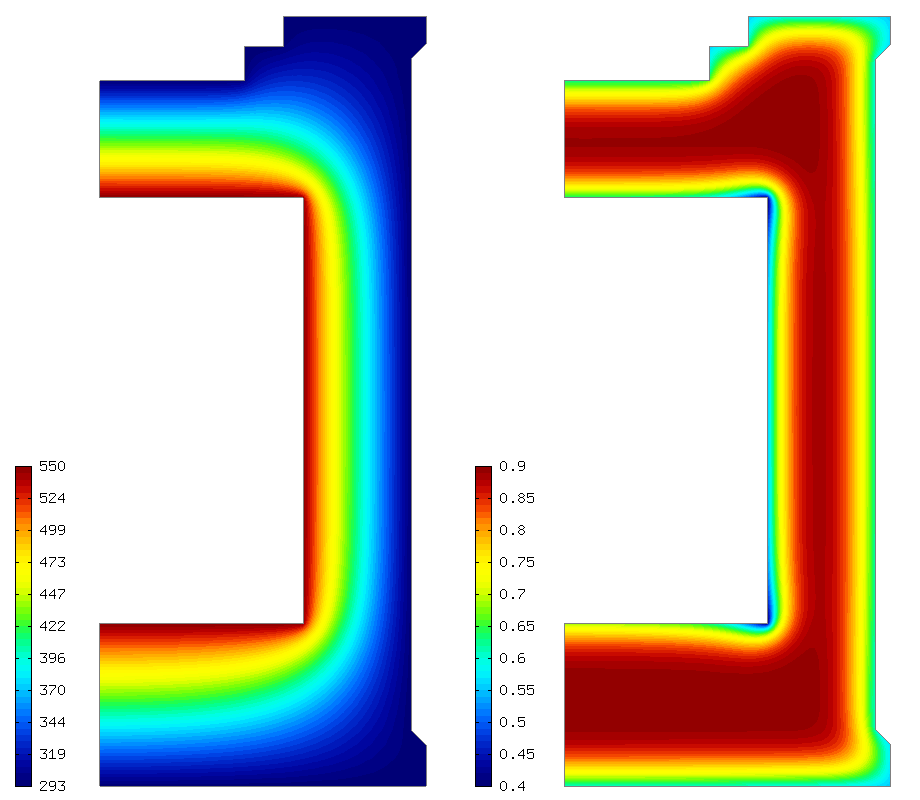
\includegraphics[height=5cm]{img/hermes_hm_sol.png}
\hspace{10mm}
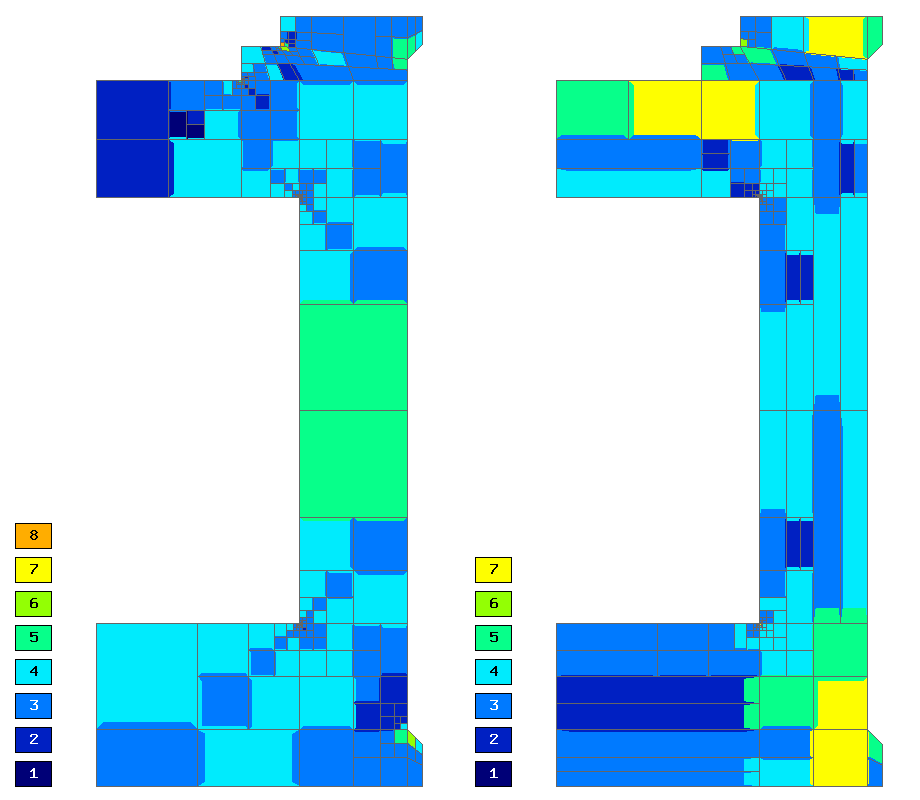
\includegraphics[height=5cm]{img/hermes_hm_mesh.png}
\caption{Illustration of multimesh hp-FEM.}
\label{fig:hermes_hm}
\end{figure}
\noindent
